\chapter{Model-Free Prediction}

Last chapter was about planning by dynamic programming. This was an approach to solving a known MDP. In many cases, however, we do not have access to the full MDP. In this case, we are talking about unknown MDPs. In this chapter, estimating the value function of an unknown MDP will be discussed.

\section{Monte-Carlo RL}

Sampling methods like Monte-Carlo methods are about learning from episodes of experience. This means they don't need to have any knowledge of the dynamics of the MDP (transitions and rewards). This makes them model-free methods. The point of MC methods is to run until the end of each episode. This means it can only work if episodes always terminate. It backtracks the experience that was generated during the episode to estimate the value function. They are based on one simple idea: \textbf{value = mean return}.\\

Walking through episodes of a problem using policy $\pi$ yields the information $S_1, A_1, R_1, ..., S_k \sim \pi$. The return is the total discounted reward, computed by $G_t = R_{t+1} + \gamma R_{t+2} + ... + \gamma^{T-1}R_T$. Then, $v_\pi(s) = \E_\pi \left[G_t | S_t = s\right]$. Instead of this \textit{expected} return, MC policy evaluation uses an \textit{empirical mean} return.\\

\begin{algorithm}[H]
	\caption{Iteration in Monte-Carlo methods}
	\label{alg:MC-eval}
	\begin{algorithmic}
		\REQUIRE policy $\pi$
		\STATE $\forall s: V(s) \Leftarrow 0, N(s) \Leftarrow 0, S(s) \Leftarrow 0$
		\FOR{$t \Leftarrow 0, ..., T$}
			\STATE $A_t, R_{t+1}, S_{t+1} \sim \pi$
			\STATE $N(S_t) \Leftarrow N(S_t) + 1$
			\STATE $S(S_t) \Leftarrow S(S_t) + G_t$
			\STATE $V(S_t) \Leftarrow \frac{S(S_t)}{N(S_t)}$
		\ENDFOR
		\RETURN $V$
	\end{algorithmic}
\end{algorithm}

By the law of large numbers
\begin{equation*}
	\lim_{N(s) \Rightarrow \infty} V(s) = v_\pi(s)
\end{equation*} 

This algorithm uses an \textit{every-visit} approach, meaning it will execute an iteration every time $S_t$ has been encountered in an episode. There is a second approach called \textit{first-visit}. This works by only doing the iteration for state $S_t$ at most once per episode, when it is encountered for the first time. 

Imagine that at time $t$ you observe $S_t$, but the same state is observed at time $t+2$. Then, $S_t = S_{t+2}$. The first-visit approach will not do the iteration at $t+2$, but the every visit will.\\

There is also a way of computing the mean incrementally.
\begin{equation*}
	\begin{aligned}
		V_t(S) & = \frac{S_t(S)}{N_t(S)}\\
			 & = \frac{1}{N_t(S)} (G_t + S_{t-1}(S))\\
			 & = \frac{1}{N_t(S)} (G_t + (N_t(S)-1)V_{t-1}(S))\\
			 & = V_{t-1}(S) + \frac{1}{N_t(S)} (G_t - V_{t-1}(S))\\
		V(S_t) & = V(S_t) + \frac{1}{N(S_t)} (G_t - V(S_t)) 
	\end{aligned}
\end{equation*}

This way you can see how it works intuitively. The current perception of the value is updated using a difference in the observed return and current perception of the value, weighted by the number of times a state is visited.\\

However, this means that we will never completely forget old experience, since we are using this moving average. In non-stationary problems, it may be useful to track the running mean to forget old episodes. This can be achieved by for example replacing $\frac{1}{N(S_t)}$ by a constant $\alpha$. The new equation will become $V(S_t) = V(S_t) + \alpha (G_t - V(S_t))$.

\section{Temporal-Difference RL}

One problem with Monte-Carlo methods is that we need episodes to terminate. TD-Learning on the other hand, does not need this. Like MC, they learn directly from episodes of experience. They are also model-free. The key difference is that TD-Learning uses a concept called \textbf{bootstrapping} to learn from incomplete episodes. They basically update towards a guess of $G_t$.\\

The simplest TD-algorithm is called TD(0). It attempts to update the value towards the estimated return $R_{t+1} + \gamma V(S_{t+1})$, which it uses as a guess for the expected return $G_t$. This value is often referred to as the TD target. Updating the value function will then become $V(S_t) = V(S_t) + \alpha (R_{t+1} + \gamma V(S_{t+1}) - V(S_t)) = V(S_t) + \alpha \delta_t$ where $\delta_t$ is referred to  as the TD error.

\section{Comparison of methods}

One big difference between TD and MC is that TD can learn \textit{online} after every step and without the final outcome. MC must wait until the episode is over, not being able to learn from incomplete/non-terminating sequences.

We know that the return $G_t = R_{t+1} + \gamma V_\pi(S_{t+1})$ is an \textit{unbiased} estimate of $v_\pi(S_t)$. TD uses a \textit{biased} estimate of the value function, since it uses $R_{t+1} + \gamma V(S_{t+1})$ to bootstrap. The positive thing about this is that the TD target has a much lower variance than the return. This is because the return depends on many random actions/transitions/rewards, while the TD target only depends on one random action/transition/reward.

Both MC and TD converge to the true value function for a policy as we get infinite experience. However, for finite batches of experience that are repeatedly sampled, they will not produce the same results.

Monte-Carlo methods converge to the solution to the best fit of the observed return. It has the objective function
\begin{equation*}
	\min \sum_{k = 1}^K \sum_{t = 1}^{T_k} (G_t^k - V(s_t^k))^2
\end{equation*}

Temporal-Difference methods on the other hand converge to the solution of the \textit{maximum likelihood Markov model}. It constructs and solves (given $\pi$) the MDP $(S, A, \hat{P}, \hat{R}, \gamma)$ that best fits the data.
\begin{equation*}
	\begin{aligned}
		& \hat{P^a_{ss'}} = \frac{1}{N(s,a)} \sum_{k = 1}^K \sum_{t = 1}^{T_k} 1(s^k_t, a^k_t, s^k_{t+1} = s, a, s')\\
		& \hat{R^a_{s}} = \frac{1}{N(s,a)} \sum_{k = 1}^K \sum_{t = 1}^{T_k} 1(s^k_t, a^k_t = s, a)r^k_t
	\end{aligned}
\end{equation*}

From this you can see TD exploits the Markov property. Standard MC does not do this. For this reason, TD is usually more effective in Markov environments and MC in non-Markov environments.

\section{TD($\lambda$)}

As we saw before, TD(0) looks one step into the future, by calculating $R_{t+1} + \gamma V(S_{t+1})$. Can we look more steps into the future? The answer is yes. For example, a 2-step TD target can be calculated as $R_{t+1} + \gamma R_{t+2} + \gamma^2 V(S_{t+2})$. It is interesting to notice that when we look $\infty$ steps into the future, we converge to the Monte-Carlo method!

In general, the $n$-step return $G^{(n)}_t = R_{t+1} + \gamma R_{t+2} + ... + \gamma^{n-1} R_{t+n} + \gamma^n V(S_{t+n})$. To perform $n$-step TD, you just use $G^{(n)}_t$ as your estimation of $G_t$.\\

We can even average different $n$-step returns to create a more sound estimate of $G_t$. For example, $\frac{1}{2} G^{(2)} + \frac{1}{2} G^{(4)}$. The idea that rises is whether we can efficiently combine information from all time-steps.\\

This is actually what TD($\lambda$) does. It defines the $\lambda$-return $G^\lambda_t$ that combines all $n$-step returns. The method uses weighting $(1 - \lambda)\lambda^{n - 1}$. The reason for this weighting is that it has nice convergence properties that allow us to calculate this return in the same time-complexity as TD(0).

We obtain $G^\lambda_t = (1-\lambda) \sum^\infty_{n = 1} \lambda^{n-1} G_t^{(n)}$. \textbf{Forward view TD($\lambda$)} will then be $V(S_t) = V(S_t) + \alpha (G^\lambda_t - V(S_t))$.

\begin{figure}[H]
	\centering
	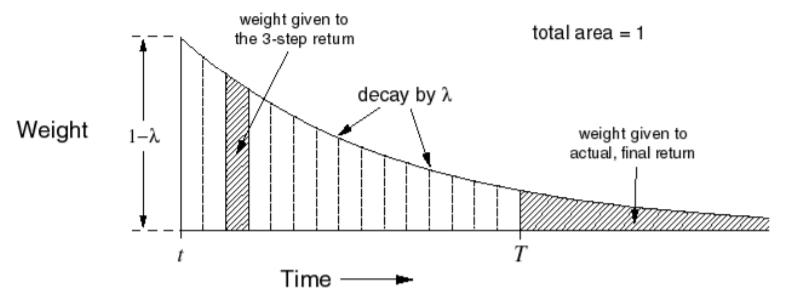
\includegraphics[width=14cm]{lambda-weighting}
	\caption{Influence of weighting on different returns $G^{(n)}$}
	\label{fig:lambda-weighting}
\end{figure}

As seen in \ref{fig:lambda-weighting}, more recent states get a higher weighting in TD($\lambda$). The weight decays as we look more into the future.\\

There is a problem with this forward-view algorithm. Just like MC, the estimated return can only be computed once the episode terminates. Luckily, there is another view for TD($\lambda$) called the \textbf{Backward View}. This algorithm allows for updating online, on every step from incomplete sequences. \\

To understand Backward View TD, lets introduce a concept called \textbf{Eligibility traces}. Imagine you're in a situation where you just got electrocuted. This happened right before you heard a bell right. Before that bell even rang, light flashed three times. What do you think caused the shock? The light flashes or the bell? 

The idea of this is that this is controlled by \textbf{Frequency heuristics} and \textbf{Recency heuristics}. We can combine both of these heuristics to form Eligibility Traces. Let $E_t(S)$ be the eligibility trace of state $s$ at time $t$. Initially, $E_0(s) = 0$. We create the recursive relationship $E_t(s) = \gamma \lambda E_{t-1}(s) + 1(S_t = s)$. Observe that at time $t$, if we're in state $s$, a value of 1 will be added to $E_t(s)$. However, for all other previously visited states, their trace only gets decayed. This corresponds to the intuition of figure \ref{fig:lambda-weighting}.\\

For Backward View TD($\lambda$), the idea is the following
\begin{itemize}
	\item Keep an eligibility trace for all states $s$
	\item Update value V(s) for every state $s$
	\item In proportion to TD-error $\delta_t$ and $E_t(s)$, we say $V(s) = V(s) + \alpha \delta_t E_t(s)$
\end{itemize}

Intuitively, this means you are constantly decaying and updating the values of previously observed states. When $\lambda = 0$, we end up with TD(0). When $\lambda = 1$, the credit is deferred until the end of the episode. This means that \textit{over the course of an episode}, the total update for TD(1) is the same as the total update for every-visit MC.

\begin{algorithm}[H]
	\caption{Iteration of TD($\lambda$)}
	\label{alg:MC-eval}
	\begin{algorithmic}
		\REQUIRE policy $\pi$
		\STATE $\forall s: V(s) \Leftarrow 0, E(s) = 0$
		\FOR{$t \Leftarrow 0, ..., T$}
		\STATE $A_t, R_{t+1}, S_{t+1} \sim \pi$
		\STATE $\delta_t \Leftarrow R_{t+1} + \gamma V(S_{t+1}) - V(S_t)$
		\STATE $E(S_t) \Leftarrow E(S_t) + 1$
			\FOR{all unique previously occurred $s$}
				\STATE $V(s) \Leftarrow V(s) + \alpha \delta_t E(s)$
				\STATE $E(s) \Leftarrow \gamma \lambda E(s)$
			\ENDFOR
		\ENDFOR
		\RETURN $V$
	\end{algorithmic}
\end{algorithm}
 